\subsection{Honeyd}
Honeyd ist ein von Niels Provos entwickelter Honeypot Deamon, der verschiedene virtuelle Host Systeme wie Workstations oder Netzwerkgeräte emulieren kann. Somit ist es möglich, eine komplette Netzstruktur zu emulieren. Die Open Source Sofware wird unter GPL veröffentlicht, und ist somit ohne Lizenzkosten benutzbar. Die aktuelle Version 1.5c wurde am 27.05.2007 veröffentlicht. Über die Benutzung von Konfigurationsdateien kann eine vielzahl von Betriebssystemen gewählt werden. Dabei werden s.g. Templates erstellt, für die zuerst eine Identität gewählt werden muss. Danach können verschiedene Parameter das simulierte Verhalten des virtuellen Clients festgelegt werden. Dazu gehören z.B. das eine emulierte Bandbreite des Übertragungskanals, Default-Aktionen verschiedener Ports und die zu aktivierenden Scripts beim Zugriff auf verschiedenen Ports. Zuletzt wird dem Template die gewünschte IP zugewiesen. In einer Honeyd Konfigurationsdatei können mehrere Clients eingetragen werden werden. Ein minimales Beispiel einer Honeyd-Konfigurationsdatei befindet sich in Abb. \ref{honeydConf}. Die Skripte, die bei einem versuchten Zugriff auf einem Port gestartet werden sollen können beliebig erstellt oder manipuliert werden. 
\\
\begin{figure}[ht]
    \centering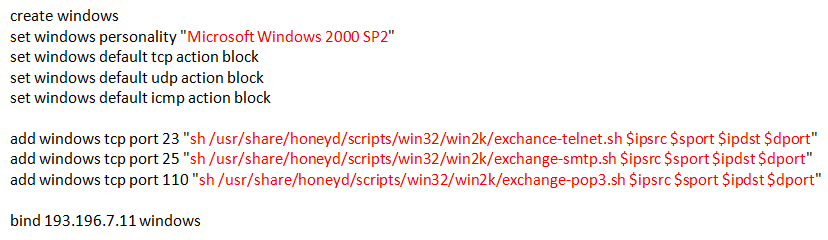
\includegraphics[scale=0.7]{Bilder/HoneydConf.png}
  \caption{Beispielkonfiguration einer Honeyd Config-Datei}
  \label{honeydConf}
\end{figure}

Honeyd wird unter Unix Systemen in der Kommandozeile ausgeführt. Dabei stellt das Programm verschiedene Konfigurationsmöglichkeiten zur Verfügung. Über den Parameter honeyd -d wird das Programm nicht als Deamon gestartet. So kann man in der Konsole nach starten des Programmes die erfolgten Zugriffe beobachten. Diese möglicherweise versuchten Angriffe (je nach Netz werden auch alle Pakete die an die Broadcast Adresse gesendet werden empfangen) müssen danach analysiert werden. Um ein möglichst leicht auswertbares Ergebnis zu erhalten kann eine feste Angabe des abzuhörenden Netzbereichs sowie die Erstellung einer Log-Datei erfolgen. Der folgende Befehl kann so auf das zuvor genannte Beispiel angewandt werden:\\
\\
\noindent\emph{honeyd -f honeyd.conf 193.196.7.11 -l honeyd.log}\\
\\
Hierbei werden nur die Pakete die für die Zieladresse 193.196.7.11 bestimmt sind für eine Auswertung in Betracht gezogen. Die erfolgten Zugriffe werden in der Datei honeyd.log gespeichert.
Die Log-Dateien speichern folgende Datensätze: \\
\\
\noindent\emph{2014-02-22-15:50:59.5296 tcp(6) S 109.193.95.133 21473 193.196.7.11 23 [Windows 2000 RFC1323]}\\
\\
Zunächst wird der Zeitpunkt des Angriffes festgestellt. Danach ob der Zugriff über TCP, UDP oder ICMP stattgefunden hat. Das S kennzeichnet den Start einer Verbindung. Bei UDP oder Paketen, die das Ende einer Verbindung kennzeichnen befindet sich an dieser Stelle ein E. Die nächsten beiden Werte sind die Quelle und Ziel IP-Adressen mit dem dazugehörigen Ports. Zuletzt befindet sich ein Versuch über Passive Fingerprinting das Betriebssystem des Angreifers zu erraten. 
Bei diesem Beispiel handelt es sich um einen Versuch über Telnet auf den Honeypot zuzugreifen. Da Honeyd seit 2007 nicht mehr weiterentwickelt wird verwendet es in diesem Beispiel eine veraltete Fingerprint Datenbank und gibt statt des verwendeten Windows 8.1 einen Windows 2000 Rechner an. 